\section{Methodology}\label{sec:lit_methodology}

This section elaborates the entire review process, from its conceptual phases to the list of selected papers and how we organized their contents, until conclusions drawing.
First, we establish the research questions that drive both the selection of papers and the data presented and discussed in subsequent sections.
Then, we explain the planning and design phase of the survey, followed by its actual execution.
We also highlight the data that was extracted from each paper and the process of sending complementary questions to authors via e-mail. We present the survey with practitioners that we conducted in support of the study conclusions.
Finally, we make available the relevant data needed to replicate this process, to the extent of possibility.

\subsection{Planning and Design of the Review}

To answer the questions above, we designed the following literature review process.
For the purposes of this review, a ``regression testing technique'' addresses test case prioritization (\tcp), test case selection (\tcs), test suite reduction (\tsr), or test suite amplification (\tsa).
Only papers concerning one or more of these four challenges should be considered.
Due to the scale of the available literature and our focused interest in recent developments, we only look for papers published between January/2016 and July/2022.
We also only consider papers written in English.

We want to focus on papers that either signify an advance of the state of the art in academia towards practicality, or includes data and discussions that might help guide future researchers to make their research more valuable for practitioners.
Thus, to be included in the review, a paper must satisfy at least one of these inclusion criteria:
\begin{itemize}
    \item It introduces a new regression testing technique and provides evidence that it addresses a real-world concern, or provides substantial benefits in experiments performed with real software;
    \item It introduces and/or discusses a metric for evaluating regression testing techniques with evidence that it might be valuable in practice; or
    \item It provides a case study of how regression testing is done in a certain team or company, and provides some insight into the actual needs of practitioners.
\end{itemize}

We also want to avoid certain topics that are related to regression testing but would increase the scope of the review beyond necessary.
A paper should be excluded according to following criteria:
\begin{itemize}
    \item It is regarding software testing education, as this is a completely different challenge;
    \item It proposes a technique for test suite generation, which is related albeit distinct problem from \tsa \footnote{The primary difference is that \textit{test suite augmentation} presupposes the existence of a test suite to enhance, while \textit{test suite generation} can create a new test suite from scratch.};
    \item It is concerning security testing, because it typically requires specific types of techniques~\cite{FELDERER20161}; or
    \item It is concerning software product lines or highly configurable software, as these also present quite different challenges from typical regression testing~\cite{do2014strategies}.
\end{itemize}

After collecting the unfiltered set of papers, the inclusion and exclusion criteria are applied by each author to a random sample set based on their titles, abstracts and, if needed, superficial analysis of the text.
In case of divergences in the analysis, the authors should discuss their conclusions.
The Cohen Kappa agreement measure~\cite{cohen1960coefficient}, a scale from -1 to 1, is used to determine if both authors are generally in agreement regarding this sample of papers.
Upon establishing a satisfying agreement value, the analysis of remaining papers are split among the authors.
If it is not clear whether a paper fully satisfies the criteria, it is brought for discussion among all authors until a mutual decision is reached.

After this initial analysis, full-text assessment of the remaining literature is performed.
The following quality criteria are to be used to further narrow down the papers that are relevant to our research goals:
\begin{itemize}
	\item The writing and presentation quality should not hinder comprehension; 
    \item A paper should provide evidence that they address a problem found in real-world software development and/or that the technique was evaluated on real-world software;
    \item The metrics used for evaluation should be clear and the authors should provide some reasoning as to why they are relevant; and
    \item In case there are multiple papers by the same group of authors that reference versions of the same work, we keep the most extensive one, avoiding, for instance, a conference paper and a journal paper that address the same research (if they are equivalent, we keep the most recent one).
\end{itemize}

The results from our queries are complemented by both forward and backward snowballing to improve the comprehensiveness of the review. 
The same date restrictions and criteria apply to papers found via snowballing.

Finally, a questionnaire with authors (\Cref{subsec:questionnaires}) is used in order to clarify and update some details regarding the selected papers.
The authors have the option of suggesting additional papers for consideration in this study; in that case, they should also be analyzed according to the established criteria.

\subsection{Executing the Review}
We began by assembling a list of keywords that form the basis of our queries, including potential variants of the same terms. 
These are: test/testing, evaluate/evaluation, metric, indicator, investment, cost, relevant/relevance, industry/industrial, practice/practical/practitioner, applicable/applicability, scale/scalability, regression, selection, prioriti[s/z]ation, amplification/augmentation, reduction/minimi[s/z]ation software.
These keywords were used to manually experiment with the ACM and IEEE digital libraries, in order to have a general understanding of the relevance of the results. 
We found, for example, that the term ``regression'' would often bring papers on the broad topic of machine learning (even not related to \rt), so we had to make sure the word ``software'' was also mentioned in the abstract.

Once the desired keywords were established, we built a query combining them.
The query went through several iterations, in order to maximize the likelihood of finding all the papers that are relevant to our research, while also minimizing the number of papers in excess.
The final query was structured as:

%\small
\begin{tcolorbox}
\small
\begin{verbatim}
Title:(test OR testing) AND 
Abstract:(evaluat* OR metric OR indicator OR investment OR cost OR relevan*) AND
Abstract:(industr* OR practic* OR applicab* OR scal*) AND
Abstract:(regression OR selection OR prioriti* OR augmentation OR 
          amplification OR reduction OR minimi*) AND
Abstract:(software)
\end{verbatim}
\end{tcolorbox}

%\normalsize


\label{subsec:execution}

\begin{table}[]
    \centering
    \begin{tabular}{cccccc}
        \toprule
        ACM & IEEE & Springer & Scopus & Wiley & \textbf{Total} \\
        \midrule
        217 & 189 & 202 & 285 & 31 & \textbf{865} \\
        \bottomrule
    \end{tabular}
    \caption{Number of results for each search engine}
    \label{tab:numberofresults}
\end{table}


Queries were executed on five digital libraries: ACM, IEEE, Springer, Scopus and Wiley.
The searches were performed on Nov. 4, 2021 and Jul. 27, 2022.
Each of the five search engines uses a different syntax for queries, so we adapted the query to each syntax while keeping its overall meaning as similar as possible.
We also attempted to include results from Science Direct into the study, but its search engine cannot handle all of the query details.
In all of the search engines, we narrowed the results to papers published since January of 2016 and under the fields of Computer Science and Software Engineering.

The number of results were: ACM (217), IEEE (189), Springer (202), Scopus (285), Wiley (31).
The total number was 865.
Removing exact duplicates that were found in more than one digital library, the number of papers considered for the review was 780.
We then assembled a spreadsheet with the year, author list, title, abstract and keywords of each paper in a shuffled order, to be reviewed by two of the authors of this study.
A sample of 40 papers was used to calculate the Cohen Kappa measure and establish a consensus.
From these, we achieved an agreement value of 0.89, which is considered very high, so we were satisfied with the criteria and the authors' interpretations of them.
Processing of the remaining papers was split among us.

This initial filtering resulted in 180 remaining papers, on which we conducted full-text analysis to ensure topic relevance and satisfaction of exclusion and quality criteria.
Like the previous step, a set of 20 papers was analyzed and discussed by all authors, and again we achieved a satisfactory agreement value; analysis of the remaining ones was split.
When there was uncertainty, some were discussed between the authors and we decided to be overly inclusive at this step, leaving the most rigorous filtering for last.
Papers from the same groups of authors were also flagged to then determine if they were describing the same or similar work.
Our list, before any snowballing, contained 86 papers.

Snowballing upon the selected primary studies was performed on Nov. 15 2021 and Aug. 15 2022, using the papers' own references for backward snowballing and Google Scholar for forward snowballing.
This resulted in a further 540 papers published since 2016, after removing duplicates of papers already found in the previous review step.
From the snowballing sample, we selected 108 candidates, forming a pool of 194 papers for analysis.

We performed full-text analysis of these papers, carefully extracting the information pointed out in \Cref{subsec:extraction} and using that to form the decision of whether or not the paper satisfied our inclusion and quality criteria.
Again during this step, we divided the papers among the authors and, in case there was uncertainty regarding one paper, we made the decision together.

Later, when we received responses from the authors of the selected studies (\Cref{subsec:questionnaires}), four papers were brought to our attention.
We applied all our aforementioned criteria to these suggestions and decided to incorporate one of them into the review.
It had not been caught by either the query or the snowballing process, but we understand that a single missed paper is evidence that our review process has been sufficiently comprehensive.

Finally, our survey, as is presented in this study, contains the \numpapers papers listed in \Cref{table:selected}: 46 found by the query; 16 from backward snowballing; 16 from forward snowballing; and 1 author suggestion.
The entire selection process is illustrated in~\Cref{fig:literature_review}.
%As is later discussed in \Cref{sec:repository}, this group of papers is just the initial contents of the live repository that is made available online.
%Over time, through updates to the review and submissions by authors, we expect this list to grow.

It is noteworthy that other studies, not included in this review, are also important for the advancement of software engineering research.
During the execution of this review, we came across several papers that provide meaningful contributions to the theory or practice of regression testing research, but exist in an isolated context.
The focus of this collection of studies is to find techniques and approaches that are applicable in real software or are close to that \-- oftentimes, these papers are the result of a longer series of smaller contributions that ultimately culminated in a usable product.

\begin{figure}
  \center
  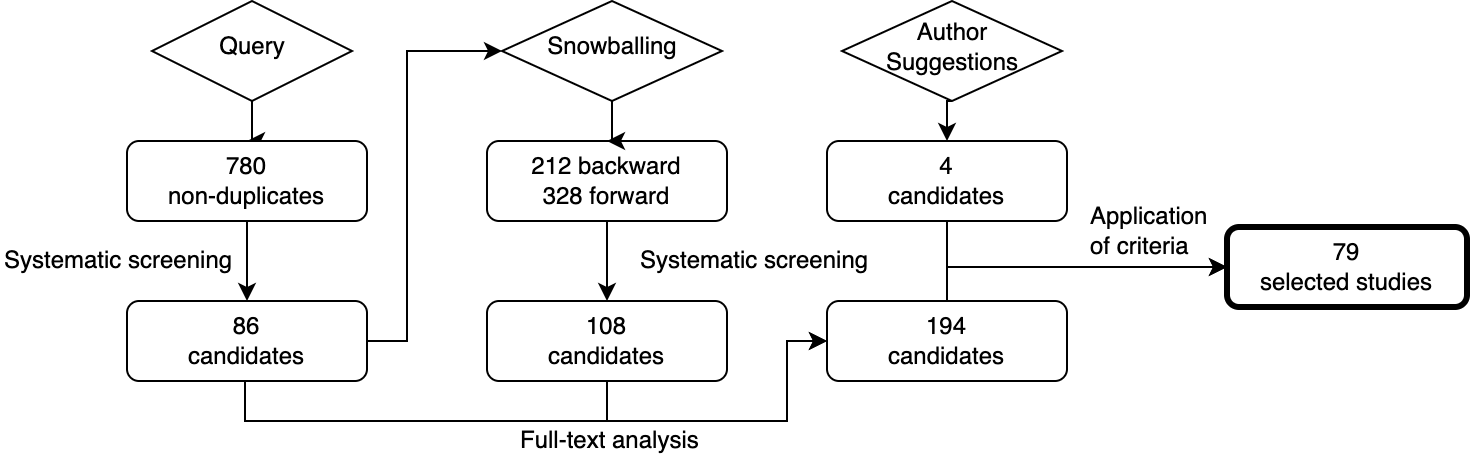
\includegraphics[width=0.8\linewidth]{figures/slr_tight.png}
  \caption{Diagram of the literature review process.}
  \label{fig:literature_review}
\end{figure}

\newcommand{\rowselected}[6]{
\scriptsize \citetalias{#1} & % Citation alias
%\scriptsize \citep{#1} & % Standard citation
\scriptsize \citeyear{#1} & % Citation year
\scriptsize \nohyphens{\citet{#1}} & % Authors
\scriptsize #2 & % Full title
\scriptsize {\color{olive} #3} & % TCP
\scriptsize {\color{teal} #4} & % TCS
\scriptsize {\color{brown} #5} & % TSR
\scriptsize {\color{purple} #6} % TSA
\tabularnewline }

%\begin{table}[]

%\begin{center}
\rowcolors{3}{}{gray!10}
\setlength{\tabcolsep}{1.2pt}
\begin{longtable}{p{5mm}lp{22mm}p{90mm}llll}
\toprule
\scriptsize \textbf{ID} & 
\scriptsize \textbf{Year} & 
\scriptsize \textbf{Authors} & 
\scriptsize \textbf{Title} & 
\scriptsize \rotatedheader{olive}{\tcp} & 
\scriptsize \rotatedheader{teal}{\tcs} &
\scriptsize \rotatedheader{brown}{\tsr} &
\scriptsize \rotatedheader{purple}{\tsa}
\tabularnewline \midrule
%\rowselected{srikanth_requirements_2016}{Requirements Based Test Prioritization Using Risk Factors}{\fullcirc}{\emptycirc}{\emptycirc}{\emptycirc}
\rowselected{noor_similarity-based_2016}{A similarity-based approach for test case prioritization using historical failure data}{\fullcirc}{\emptycirc}{\emptycirc}{\emptycirc}
\rowselected{schwartz_cost-effective_2016}{Cost-effective regression testing through adaptive test prioritization strategies}{\fullcirc}{\emptycirc}{\emptycirc}{\emptycirc}
\rowselected{hirzel_graph-walk-based_2016}{Graph-walk-based selective regression testing of web applications created with Google web toolkit}{\emptycirc}{\fullcirc}{\emptycirc}{\emptycirc}
\rowselected{lu_how_2016}{How does regression test prioritization perform in real-world software evolution?}{\fullcirc}{\emptycirc}{\emptycirc}{\emptycirc}
\rowselected{vost_trace-based_2016}{Trace-based test selection to support continuous integration in the automotive industry}{\emptycirc}{\fullcirc}{\emptycirc}{\emptycirc}
\rowselected{wang_enhancing_2016}{Enhancing test case prioritization in an industrial setting with resource awareness and multi-objective search}{\fullcirc}{\emptycirc}{\emptycirc}{\emptycirc}
\rowselected{srikanth_test_2016}{Test Case Prioritization of Build Acceptance Tests for an Enterprise Cloud Application}{\fullcirc}{\emptycirc}{\emptycirc}{\emptycirc}
\rowselected{blondeau_test_2017}{Test case selection in industry: an analysis of issues related to static approaches}{\emptycirc}{\fullcirc}{\emptycirc}{\emptycirc}
\rowselected{pradhan_search-based_2016}{Search-Based Cost-Effective Test Case Selection within a Time Budget: An Empirical Study}{\emptycirc}{\fullcirc}{\emptycirc}{\emptycirc}
\rowselected{buchgeher_improving_2016}{Improving testing in an enterprise SOA with an architecture-based approach}{\fullcirc}{\fullcirc}{\emptycirc}{\emptycirc}
\rowselected{tahvili_dynamic_2016}{Dynamic integration test selection based on test case dependencies}{\fullcirc}{\fullcirc}{\emptycirc}{\emptycirc}
\rowselected{oqvist_extraction-based_2016}{Extraction-based regression test selection}{\emptycirc}{\fullcirc}{\emptycirc}{\emptycirc}
\rowselected{magalhaes_automatic_2016}{Automatic selection of test cases for regression testing}{\emptycirc}{\fullcirc}{\emptycirc}{\emptycirc}
\rowselected{aman_application_2016}{Application of Mahalanobis-Taguchi Method and 0-1 Programming Method to Cost-Effective Regression Testing}{\fullcirc}{\emptycirc}{\emptycirc}{\emptycirc}
\rowselected{busjaeger_learning_2016}{Learning for test prioritization: An industrial case study}{\fullcirc}{\emptycirc}{\emptycirc}{\emptycirc}
\rowselected{yoshida_fsx_2016}{FSX: A tool for fine-grained incremental unit test generation for C/C++ Programs}{\emptycirc}{\emptycirc}{\emptycirc}{\fullcirc}
\rowselected{tahvili_cost-benefit_2016}{Cost-benefit analysis of using dependency knowledge at integration testing}{\fullcirc}{\emptycirc}{\emptycirc}{\emptycirc}
\rowselected{ramler_tool_2017}{Tool support for change-based regression testing: An industry experience report}{\emptycirc}{\fullcirc}{\emptycirc}{\emptycirc}
\rowselected{strandberg_experience_2016}{Experience Report: Automated System Level Regression Test Prioritization Using Multiple Factors}{\fullcirc}{\fullcirc}{\emptycirc}{\emptycirc}
\rowselected{marijan_effect_2016}{Effect of time window on the performance of continuous regression testing}{\fullcirc}{\emptycirc}{\emptycirc}{\emptycirc}
\rowselected{gotlieb_using_2017}{Using global constraints to automate regression testing}{\emptycirc}{\emptycirc}{\fullcirc}{\emptycirc}
\rowselected{chi_multi-level_2017}{Multi-Level Random Walk for Software Test Suite Reduction}{\emptycirc}{\emptycirc}{\fullcirc}{\emptycirc}
\rowselected{bach_coverage-based_2017}{Coverage-Based Reduction of Test Execution Time: Lessons from a Very Large Industrial Project}{\fullcirc}{\fullcirc}{\emptycirc}{\emptycirc}
\rowselected{spieker_reinforcement_2017}{Reinforcement learning for automatic test case prioritization and selection in continuous integration}{\fullcirc}{\fullcirc}{\emptycirc}{\emptycirc}
\rowselected{vasic_file-level_2017}{File-Level vs. Module-Level Regression Test Selection for .NET}{\emptycirc}{\fullcirc}{\emptycirc}{\emptycirc}
\rowselected{celik_regression_2017}{Regression test selection across JVM boundaries}{\emptycirc}{\fullcirc}{\emptycirc}{\emptycirc}
\rowselected{ouriques_test_2018}{Test case prioritization techniques for model-based testing: a replicated study}{\fullcirc}{\emptycirc}{\emptycirc}{\emptycirc}
\rowselected{kwon_cost-effective_2017}{Cost-effective regression testing using bloom filters in continuous integration development environments}{\fullcirc}{\fullcirc}{\emptycirc}{\emptycirc}
\rowselected{garousi_multi-objective_2018}{Multi-objective regression test selection in practice: An empirical study in the defense software industry}{\emptycirc}{\fullcirc}{\emptycirc}{\emptycirc}
\rowselected{shi_evaluating_2018}{Evaluating test-suite reduction in real software evolution}{\emptycirc}{\emptycirc}{\fullcirc}{\emptycirc}
\rowselected{haghighatkhah_test_2018}{Test prioritization in continuous integration environments}{\fullcirc}{\emptycirc}{\emptycirc}{\emptycirc}
\rowselected{zhang_hybrid_2018}{Hybrid regression test selection}{\emptycirc}{\fullcirc}{\emptycirc}{\emptycirc}
\rowselected{miranda_fast_2018}{FAST Approaches to Scalable Similarity-Based Test Case Prioritization}{\fullcirc}{\emptycirc}{\emptycirc}{\emptycirc}
\rowselected{yilmaz_case_2018}{A case study to compare regression test selection techniques on open-source software projects}{\emptycirc}{\fullcirc}{\emptycirc}{\emptycirc}
\rowselected{chen_optimizing_2018}{Optimizing Test Prioritization via Test Distribution Analysis}{\fullcirc}{\emptycirc}{\emptycirc}{\emptycirc}
\rowselected{celik_regression_2018}{Regression Test Selection for TizenRT}{\emptycirc}{\fullcirc}{\emptycirc}{\emptycirc}
\rowselected{zhu_test_2018}{Test re-prioritization in continuous testing environments}{\fullcirc}{\emptycirc}{\emptycirc}{\emptycirc}
\rowselected{azizi_retest_2018}{Retest: A cost effective test case selection technique for modern software development}{\emptycirc}{\fullcirc}{\emptycirc}{\emptycirc}
\rowselected{guo_decomposing_2019}{Decomposing Composite Changes for Code Review and Regression Test Selection in Evolving Software}{\emptycirc}{\fullcirc}{\emptycirc}{\emptycirc}
\rowselected{zhong_testsage:_2019}{TestSage: Regression test selection for large-scale Web service testing}{\emptycirc}{\fullcirc}{\emptycirc}{\emptycirc}
\rowselected{fu_resurgence_2019}{Resurgence of Regression Test Selection for C++}{\emptycirc}{\fullcirc}{\emptycirc}{\emptycirc}
\rowselected{eda_efficient_2019}{An efficient regression testing approach for PHP Web applications using test selection and reusable constraints}{\emptycirc}{\fullcirc}{\fullcirc}{\emptycirc}
\rowselected{goyal_test_2019}{Test suite minimization of evolving software systems: A case study}{\emptycirc}{\emptycirc}{\fullcirc}{\emptycirc}
\rowselected{yu_terminator_2019}{TERMINATOR: better automated UI test case prioritization}{\fullcirc}{\emptycirc}{\emptycirc}{\emptycirc}
\rowselected{correia_motsd_2019}{MOTSD: A multi-objective test selection tool using test suite diagnosability}{\fullcirc}{\fullcirc}{\emptycirc}{\emptycirc}
\rowselected{machalica_predictive_2018}{Predictive Test Selection}{\emptycirc}{\fullcirc}{\emptycirc}{\emptycirc}
\rowselected{najafi_improving_2019}{Improving Test Effectiveness Using Test Executions History: An Industrial Experience Report}{\fullcirc}{\fullcirc}{\emptycirc}{\emptycirc}
\rowselected{leong_assessing_2019}{Assessing Transition-Based Test Selection Algorithms at Google}{\emptycirc}{\fullcirc}{\emptycirc}{\emptycirc}
\rowselected{cruciani_scalable_2019}{Scalable Approaches for Test Suite Reduction}{\emptycirc}{\emptycirc}{\fullcirc}{\emptycirc}
\rowselected{philip_fastlane:_2019}{FastLane: Test Minimization for Rapidly Deployed Large-Scale Online Services}{\emptycirc}{\emptycirc}{\fullcirc}{\emptycirc}
\rowselected{magalhaes_hsp_2020}{HSP: A hybrid selection and prioritisation of regression test cases based on information retrieval and code coverage applied on an industrial case study}{\fullcirc}{\fullcirc}{\emptycirc}{\emptycirc}
\rowselected{wu_time_2019}{A Time Window Based Reinforcement Learning Reward for Test Case Prioritization in Continuous Integration}{\fullcirc}{\emptycirc}{\emptycirc}{\emptycirc}
\rowselected{land_industrial_2019}{An Industrial Evaluation of Test Prioritisation Criteria and Metrics}{\fullcirc}{\emptycirc}{\emptycirc}{\emptycirc}
\rowselected{noemmer_evaluation_2020}{An Evaluation of Test Suite Minimization Techniques}{\emptycirc}{\emptycirc}{\fullcirc}{\emptycirc}
\rowselected{lubke_selecting_2020}{Selecting and Prioritizing Regression Test Suites by Production Usage Risk in Time-Constrained Environments}{\fullcirc}{\fullcirc}{\emptycirc}{\emptycirc}
\rowselected{yackley_simultaneous_2019}{Simultaneous refactoring and regression testing}{\emptycirc}{\fullcirc}{\emptycirc}{\emptycirc}
\rowselected{shi_understanding_2019}{Understanding and improving regression test selection in continuous integration}{\emptycirc}{\fullcirc}{\emptycirc}{\emptycirc}
\rowselected{lima_multi-armed_2022}{A Multi-Armed Bandit Approach for Test Case Prioritization in Continuous Integration Environments}{\fullcirc}{\emptycirc}{\emptycirc}{\emptycirc}
\rowselected{zhou_beating_2020}{Beating Random Test Case Prioritization}{\fullcirc}{\emptycirc}{\emptycirc}{\emptycirc}
\rowselected{peng_empirically_2020}{Empirically revisiting and enhancing IR-based test-case prioritization}{\fullcirc}{\emptycirc}{\emptycirc}{\emptycirc}
\rowselected{bertolino_learning--rank_2020}{Learning-to-rank vs ranking-to-learn: Strategies for regression testing in continuous integration}{\fullcirc}{\fullcirc}{\emptycirc}{\emptycirc}
\rowselected{chen_multi-objective_2021}{Multi-objective regression test selection}{\emptycirc}{\fullcirc}{\emptycirc}{\emptycirc}
\rowselected{zarges_artificial_2021}{An Artificial Immune System for Black Box Test Case Selection}{\emptycirc}{\emptycirc}{\emptycirc}{\emptycirc}
\rowselected{bagherzadeh_reinforcement_2022}{Reinforcement learning for test case prioritization}{\fullcirc}{\emptycirc}{\emptycirc}{\emptycirc}
\rowselected{elsner_empirically_2021}{Empirically evaluating readily available information for regression test optimization in continuous integration}{\fullcirc}{\fullcirc}{\emptycirc}{\emptycirc}
\rowselected{pan_dynamic_2020}{Dynamic Time Window based Reward for Reinforcement Learning in Continuous Integration Testing}{\fullcirc}{\emptycirc}{\emptycirc}{\emptycirc}
\rowselected{mehta_data-driven_2021}{Data-driven test selection at scale}{\emptycirc}{\fullcirc}{\emptycirc}{\emptycirc}
\rowselected{xu_requirement-based_2021}{A Requirement-based Regression Test Selection Technique in Behavior-Driven Development}{\emptycirc}{\fullcirc}{\emptycirc}{\emptycirc}
\rowselected{zhou_parallel_2022}{Parallel Test Prioritization}{\fullcirc}{\emptycirc}{\emptycirc}{\emptycirc}
\rowselected{sharif_deeporder_2021}{DeepOrder: Deep Learning for Test Case Prioritization in Continuous Integration Testing}{\fullcirc}{\emptycirc}{\emptycirc}{\emptycirc}
\rowselected{li_aga_2021}{AGA: An Accelerated Greedy Additional Algorithm for Test Case Prioritization}{\fullcirc}{\emptycirc}{\emptycirc}{\emptycirc}
\rowselected{chen_context-aware_2021}{Context-Aware Regression Test Selection}{\emptycirc}{\fullcirc}{\emptycirc}{\emptycirc}
\rowselected{zhang_comparing_2022}{Comparing and Combining Analysis-Based and Learning-Based Regression Test Selection}{\emptycirc}{\fullcirc}{\emptycirc}{\emptycirc}
\rowselected{abdelkarim_tcp-net_2022}{TCP-Net: Test Case Prioritization using End-to-End Deep Neural Networks}{\fullcirc}{\emptycirc}{\emptycirc}{\emptycirc}
\rowselected{cingil_black-box_2022}{Black-box Test Case Selection by Relating Code Changes with Previously Fixed Defects}{\emptycirc}{\fullcirc}{\emptycirc}{\emptycirc}
\rowselected{yaraghi_scalable_2022}{Scalable and Accurate Test Case Prioritization in Continuous Integration Contexts}{\fullcirc}{\emptycirc}{\emptycirc}{\emptycirc}
\rowselected{omri_learning_2022}{Learning to Rank for Test Case Prioritization}{\fullcirc}{\emptycirc}{\emptycirc}{\emptycirc}
\rowselected{greca_comparing_2022}{Comparing and combining file-based selection and similarity-based prioritization towards regression test orchestration}{\fullcirc}{\fullcirc}{\emptycirc}{\emptycirc}
\hiderowcolors
\midrule
& & & Totals & 46 & 41 & 8 & 1 
 \\ \bottomrule
\caption{Selected papers.}


\rowselected{srikanth_requirements_2016}{Requirements Based Test Prioritization Using Risk Factors}{\fullcirc}{\emptycirc}{\emptycirc}{\emptycirc}
\rowselected{noor_similarity-based_2016}{A similarity-based approach for test case prioritization using historical failure data}{\fullcirc}{\emptycirc}{\emptycirc}{\emptycirc}
\rowselected{schwartz_cost-effective_2016}{Cost-effective regression testing through adaptive test prioritization strategies}{\fullcirc}{\emptycirc}{\emptycirc}{\emptycirc}
\rowselected{hirzel_graph-walk-based_2016}{Graph-walk-based selective regression testing of web applications created with Google web toolkit}{\emptycirc}{\fullcirc}{\emptycirc}{\emptycirc}
\rowselected{lu_how_2016}{How does regression test prioritization perform in real-world software evolution?}{\fullcirc}{\emptycirc}{\emptycirc}{\emptycirc}
\rowselected{vost_trace-based_2016}{Trace-based test selection to support continuous integration in the automotive industry}{\emptycirc}{\fullcirc}{\emptycirc}{\emptycirc}
\rowselected{wang_enhancing_2016}{Enhancing test case prioritization in an industrial setting with resource awareness and multi-objective search}{\fullcirc}{\emptycirc}{\emptycirc}{\emptycirc}
\rowselected{srikanth_test_2016}{Test Case Prioritization of Build Acceptance Tests for an Enterprise Cloud Application}{\fullcirc}{\emptycirc}{\emptycirc}{\emptycirc}
\rowselected{blondeau_test_2017}{Test case selection in industry: an analysis of issues related to static approaches}{\emptycirc}{\fullcirc}{\emptycirc}{\emptycirc}
\rowselected{pradhan_search-based_2016}{Search-Based Cost-Effective Test Case Selection within a Time Budget: An Empirical Study}{\emptycirc}{\fullcirc}{\emptycirc}{\emptycirc}
\rowselected{buchgeher_improving_2016}{Improving testing in an enterprise SOA with an architecture-based approach}{\fullcirc}{\fullcirc}{\emptycirc}{\emptycirc}
\rowselected{tahvili_dynamic_2016}{Dynamic integration test selection based on test case dependencies}{\fullcirc}{\fullcirc}{\emptycirc}{\emptycirc}
\rowselected{oqvist_extraction-based_2016}{Extraction-based regression test selection}{\emptycirc}{\fullcirc}{\emptycirc}{\emptycirc}
\rowselected{magalhaes_automatic_2016}{Automatic selection of test cases for regression testing}{\emptycirc}{\fullcirc}{\emptycirc}{\emptycirc}
\rowselected{aman_application_2016}{Application of Mahalanobis-Taguchi Method and 0-1 Programming Method to Cost-Effective Regression Testing}{\fullcirc}{\emptycirc}{\emptycirc}{\emptycirc}
\rowselected{busjaeger_learning_2016}{Learning for test prioritization: An industrial case study}{\fullcirc}{\emptycirc}{\emptycirc}{\emptycirc}
\rowselected{yoshida_fsx_2016}{FSX: A tool for fine-grained incremental unit test generation for C/C++ Programs}{\emptycirc}{\emptycirc}{\emptycirc}{\fullcirc}
\rowselected{tahvili_cost-benefit_2016}{Cost-benefit analysis of using dependency knowledge at integration testing}{\fullcirc}{\emptycirc}{\emptycirc}{\emptycirc}
\rowselected{ramler_tool_2017}{Tool support for change-based regression testing: An industry experience report}{\emptycirc}{\fullcirc}{\emptycirc}{\emptycirc}
\rowselected{strandberg_experience_2016}{Experience Report: Automated System Level Regression Test Prioritization Using Multiple Factors}{\fullcirc}{\fullcirc}{\emptycirc}{\emptycirc}
\rowselected{marijan_effect_2016}{Effect of time window on the performance of continuous regression testing}{\fullcirc}{\emptycirc}{\emptycirc}{\emptycirc}
\rowselected{gotlieb_using_2017}{Using global constraints to automate regression testing}{\emptycirc}{\emptycirc}{\fullcirc}{\emptycirc}
\rowselected{chi_multi-level_2017}{Multi-Level Random Walk for Software Test Suite Reduction}{\emptycirc}{\emptycirc}{\fullcirc}{\emptycirc}
\rowselected{bach_coverage-based_2017}{Coverage-Based Reduction of Test Execution Time: Lessons from a Very Large Industrial Project}{\fullcirc}{\fullcirc}{\emptycirc}{\emptycirc}
\rowselected{spieker_reinforcement_2017}{Reinforcement learning for automatic test case prioritization and selection in continuous integration}{\fullcirc}{\fullcirc}{\emptycirc}{\emptycirc}
\rowselected{vasic_file-level_2017}{File-Level vs. Module-Level Regression Test Selection for .NET}{\emptycirc}{\fullcirc}{\emptycirc}{\emptycirc}
\rowselected{celik_regression_2017}{Regression test selection across JVM boundaries}{\emptycirc}{\fullcirc}{\emptycirc}{\emptycirc}
\rowselected{ouriques_test_2018}{Test case prioritization techniques for model-based testing: a replicated study}{\fullcirc}{\emptycirc}{\emptycirc}{\emptycirc}
\rowselected{kwon_cost-effective_2017}{Cost-effective regression testing using bloom filters in continuous integration development environments}{\fullcirc}{\fullcirc}{\emptycirc}{\emptycirc}
\rowselected{garousi_multi-objective_2018}{Multi-objective regression test selection in practice: An empirical study in the defense software industry}{\emptycirc}{\fullcirc}{\emptycirc}{\emptycirc}
\rowselected{shi_evaluating_2018}{Evaluating test-suite reduction in real software evolution}{\emptycirc}{\emptycirc}{\fullcirc}{\emptycirc}
\rowselected{haghighatkhah_test_2018}{Test prioritization in continuous integration environments}{\fullcirc}{\emptycirc}{\emptycirc}{\emptycirc}
\rowselected{zhang_hybrid_2018}{Hybrid regression test selection}{\emptycirc}{\fullcirc}{\emptycirc}{\emptycirc}
\rowselected{miranda_fast_2018}{FAST Approaches to Scalable Similarity-Based Test Case Prioritization}{\fullcirc}{\emptycirc}{\emptycirc}{\emptycirc}
\rowselected{yilmaz_case_2018}{A case study to compare regression test selection techniques on open-source software projects}{\emptycirc}{\fullcirc}{\emptycirc}{\emptycirc}
\rowselected{chen_optimizing_2018}{Optimizing Test Prioritization via Test Distribution Analysis}{\fullcirc}{\emptycirc}{\emptycirc}{\emptycirc}
\rowselected{celik_regression_2018}{Regression Test Selection for TizenRT}{\emptycirc}{\fullcirc}{\emptycirc}{\emptycirc}
\rowselected{zhu_test_2018}{Test re-prioritization in continuous testing environments}{\fullcirc}{\emptycirc}{\emptycirc}{\emptycirc}
\rowselected{azizi_retest_2018}{Retest: A cost effective test case selection technique for modern software development}{\emptycirc}{\fullcirc}{\emptycirc}{\emptycirc}
\rowselected{guo_decomposing_2019}{Decomposing Composite Changes for Code Review and Regression Test Selection in Evolving Software}{\emptycirc}{\fullcirc}{\emptycirc}{\emptycirc}
\rowselected{zhong_testsage:_2019}{TestSage: Regression test selection for large-scale Web service testing}{\emptycirc}{\fullcirc}{\emptycirc}{\emptycirc}
\rowselected{fu_resurgence_2019}{Resurgence of Regression Test Selection for C++}{\emptycirc}{\fullcirc}{\emptycirc}{\emptycirc}
\rowselected{eda_efficient_2019}{An efficient regression testing approach for PHP Web applications using test selection and reusable constraints}{\emptycirc}{\fullcirc}{\fullcirc}{\emptycirc}
\rowselected{goyal_test_2019}{Test suite minimization of evolving software systems: A case study}{\emptycirc}{\emptycirc}{\fullcirc}{\emptycirc}
\rowselected{yu_terminator_2019}{TERMINATOR: better automated UI test case prioritization}{\fullcirc}{\emptycirc}{\emptycirc}{\emptycirc}
\rowselected{correia_motsd_2019}{MOTSD: A multi-objective test selection tool using test suite diagnosability}{\fullcirc}{\fullcirc}{\emptycirc}{\emptycirc}
\rowselected{machalica_predictive_2018}{Predictive Test Selection}{\emptycirc}{\fullcirc}{\emptycirc}{\emptycirc}
\rowselected{najafi_improving_2019}{Improving Test Effectiveness Using Test Executions History: An Industrial Experience Report}{\fullcirc}{\fullcirc}{\emptycirc}{\emptycirc}
\rowselected{leong_assessing_2019}{Assessing Transition-Based Test Selection Algorithms at Google}{\emptycirc}{\fullcirc}{\emptycirc}{\emptycirc}
\rowselected{cruciani_scalable_2019}{Scalable Approaches for Test Suite Reduction}{\emptycirc}{\emptycirc}{\fullcirc}{\emptycirc}
\rowselected{philip_fastlane:_2019}{FastLane: Test Minimization for Rapidly Deployed Large-Scale Online Services}{\emptycirc}{\emptycirc}{\fullcirc}{\emptycirc}
\rowselected{magalhaes_hsp_2020}{HSP: A hybrid selection and prioritisation of regression test cases based on information retrieval and code coverage applied on an industrial case study}{\fullcirc}{\fullcirc}{\emptycirc}{\emptycirc}
\rowselected{wu_time_2019}{A Time Window Based Reinforcement Learning Reward for Test Case Prioritization in Continuous Integration}{\fullcirc}{\emptycirc}{\emptycirc}{\emptycirc}
\rowselected{land_industrial_2019}{An Industrial Evaluation of Test Prioritisation Criteria and Metrics}{\fullcirc}{\emptycirc}{\emptycirc}{\emptycirc}
\rowselected{noemmer_evaluation_2020}{An Evaluation of Test Suite Minimization Techniques}{\emptycirc}{\emptycirc}{\fullcirc}{\emptycirc}
\rowselected{lubke_selecting_2020}{Selecting and Prioritizing Regression Test Suites by Production Usage Risk in Time-Constrained Environments}{\fullcirc}{\fullcirc}{\emptycirc}{\emptycirc}
\rowselected{yackley_simultaneous_2019}{Simultaneous refactoring and regression testing}{\emptycirc}{\fullcirc}{\emptycirc}{\emptycirc}
\rowselected{shi_understanding_2019}{Understanding and improving regression test selection in continuous integration}{\emptycirc}{\fullcirc}{\emptycirc}{\emptycirc}
\rowselected{lima_multi-armed_2022}{A Multi-Armed Bandit Approach for Test Case Prioritization in Continuous Integration Environments}{\fullcirc}{\emptycirc}{\emptycirc}{\emptycirc}
\rowselected{zhou_beating_2020}{Beating Random Test Case Prioritization}{\fullcirc}{\emptycirc}{\emptycirc}{\emptycirc}
\rowselected{peng_empirically_2020}{Empirically revisiting and enhancing IR-based test-case prioritization}{\fullcirc}{\emptycirc}{\emptycirc}{\emptycirc}
\rowselected{bertolino_learning--rank_2020}{Learning-to-rank vs ranking-to-learn: Strategies for regression testing in continuous integration}{\fullcirc}{\fullcirc}{\emptycirc}{\emptycirc}
\rowselected{chen_multi-objective_2021}{Multi-objective regression test selection}{\emptycirc}{\fullcirc}{\emptycirc}{\emptycirc}
\rowselected{zarges_artificial_2021}{An Artificial Immune System for Black Box Test Case Selection}{\emptycirc}{\emptycirc}{\emptycirc}{\emptycirc}
\rowselected{bagherzadeh_reinforcement_2022}{Reinforcement learning for test case prioritization}{\fullcirc}{\emptycirc}{\emptycirc}{\emptycirc}
\rowselected{elsner_empirically_2021}{Empirically evaluating readily available information for regression test optimization in continuous integration}{\fullcirc}{\fullcirc}{\emptycirc}{\emptycirc}
\rowselected{pan_dynamic_2020}{Dynamic Time Window based Reward for Reinforcement Learning in Continuous Integration Testing}{\fullcirc}{\emptycirc}{\emptycirc}{\emptycirc}
\rowselected{mehta_data-driven_2021}{Data-driven test selection at scale}{\emptycirc}{\fullcirc}{\emptycirc}{\emptycirc}
\rowselected{xu_requirement-based_2021}{A Requirement-based Regression Test Selection Technique in Behavior-Driven Development}{\emptycirc}{\fullcirc}{\emptycirc}{\emptycirc}
\rowselected{zhou_parallel_2022}{Parallel Test Prioritization}{\fullcirc}{\emptycirc}{\emptycirc}{\emptycirc}
\rowselected{sharif_deeporder_2021}{DeepOrder: Deep Learning for Test Case Prioritization in Continuous Integration Testing}{\fullcirc}{\emptycirc}{\emptycirc}{\emptycirc}
\rowselected{li_aga_2021}{AGA: An Accelerated Greedy Additional Algorithm for Test Case Prioritization}{\fullcirc}{\emptycirc}{\emptycirc}{\emptycirc}
\rowselected{chen_context-aware_2021}{Context-Aware Regression Test Selection}{\emptycirc}{\fullcirc}{\emptycirc}{\emptycirc}
\rowselected{zhang_comparing_2022}{Comparing and Combining Analysis-Based and Learning-Based Regression Test Selection}{\emptycirc}{\fullcirc}{\emptycirc}{\emptycirc}
\rowselected{abdelkarim_tcp-net_2022}{TCP-Net: Test Case Prioritization using End-to-End Deep Neural Networks}{\fullcirc}{\emptycirc}{\emptycirc}{\emptycirc}
\rowselected{cingil_black-box_2022}{Black-box Test Case Selection by Relating Code Changes with Previously Fixed Defects}{\emptycirc}{\fullcirc}{\emptycirc}{\emptycirc}
\rowselected{yaraghi_scalable_2022}{Scalable and Accurate Test Case Prioritization in Continuous Integration Contexts}{\fullcirc}{\emptycirc}{\emptycirc}{\emptycirc}
\rowselected{omri_learning_2022}{Learning to Rank for Test Case Prioritization}{\fullcirc}{\emptycirc}{\emptycirc}{\emptycirc}
\rowselected{greca_comparing_2022}{Comparing and combining file-based selection and similarity-based prioritization towards regression test orchestration}{\fullcirc}{\fullcirc}{\emptycirc}{\emptycirc}
\hiderowcolors
\midrule
& & & Totals & 46 & 41 & 8 & 1 
 \\ \bottomrule
\caption{Selected papers.}

%\\
%\hiderowcolors
%\bottomrule
%\caption{Selected papers.}
\label{table:selected}
\end{longtable}
%\end{center}

\setlength{\tabcolsep}{6pt}

%\begin{table}[]
%\centering
%\scriptsize
%\rowcolors{1}{}{gray!10}
%\begin{tabular}{llp{40mm}p{60mm}ll}
%\toprule
%\textbf{ID} & \textbf{Year} & \textbf{Authors} & \textbf{Title} & \textbf{Publisher} & \textbf{Ref.}  \\ \midrule
%%\input{tables/csv_selected_1.tex}
%%\rowselected{srikanth_requirements_2016}{Requirements Based Test Prioritization Using Risk Factors}{Elsevier}
%
%\bottomrule
%\end{tabular}
%%\caption{Selected papers.}
%\label{table:selected_1}
%\end{table}
%
%\begin{table}[]
%\centering
%\scriptsize
%\rowcolors{1}{}{gray!10}
%\begin{tabular}{llp{40mm}p{60mm}ll}
%\toprule
%\textbf{ID} & \textbf{Year} & \textbf{Authors} & \textbf{Title} & \textbf{Publisher} & \textbf{Ref.}  \\ \midrule
%\input{csv_selected_2.tex}
%\bottomrule
%\end{tabular}
%%\caption{Selected papers.}
%\label{table:selected_2}
%\end{table}
%
%\begin{table}[]
%\centering
%\scriptsize
%\rowcolors{1}{}{gray!10}
%\begin{tabular}{llp{40mm}p{60mm}ll}
%\toprule
%\textbf{ID} & \textbf{Year} & \textbf{Authors} & \textbf{Title} & \textbf{Publisher} & \textbf{Ref.}  \\ \midrule
%\input{csv_selected_3.tex}
%\bottomrule
%\end{tabular}
%\caption{Selected papers.}
%\label{table:selected_3}
%\end{table}

\subsection{Data Extraction}
\label{subsec:extraction}


To collect the data, each of the selected papers was assigned to one author to lead the data extraction, and to another author to review the data afterwards.
Thus, each paper was thoroughly reviewed by at least two authors.
At the end of this phase, the three authors performed a broad review of the collected information in order to ensure consistency of the results.

During the full-text analysis of the selected papers, we took notes of four groups of properties we wished to extract from each paper.
First, we wanted to have the core bibliographical information of the paper.
Then, we categorized the papers according to the \rt challenge being addressed and contextual factors such as software type and development environment.
We also took note of eight properties we considered important regarding \rea of each proposed technique or case study.
Finally, we synthesized the results of the papers by highlighting the types of approaches and metrics used and, if available, the open challenges/future work discussed by the authors.
The properties we collected are listed in \Cref{table:extraction}.

Some further explanation is needed regarding the ``applicability concerns'' properties.
During the data extraction, it became clear to us that there is some ambiguity regarding industrial motivation; among the non-selected papers, we also saw a great number of them briefly mentioning industry needs in the abstract and introduction, but not forming a connection between those needs and the technique being proposed.
So, for our criteria, industrial needs must not only be mentioned, but clearly stated with motivating evidence and/or references, and serve as the actual principle behind the idea of the study.

Regarding the industrial evaluation of results, this property is satisfied when experiments are performed directly on industrial software, usually through collaboration with a technology company.
However, there are plenty of papers that have robust experiments performed on notable open-source software, such as those from the Apache and Mozilla foundations.
Thus, we collect the following information about the subjects:
\begin{itemize}
	\item Its openness, which can be industrial proprietary, industrial open-source, fully open-source, or an academic dataset;
	\item Its testing scale (small up to 500 TCs, medium up to 2,000 TCs, large up to 10,000 TCs, or very large if more than that)\footnote{It is also important to note that the number of test cases is only one dimension of scale: on~\citetalias{cingil_black-box_2022}, for example, evaluation was performed on Smart TV apps with only 38 test cases, but the testing time was over 7 hours.};
	\item The language used for writing tests, which can be a programming language, natural language, a domain-specific language or a combination; and
	\item Its origin (the company that wrote it, or the dataset it is from).
\end{itemize}

We also checked to see if there is feedback from practitioners in the text of the paper.
Relatively few authors include feedback and, often times, it is only a brief passage.
Sometimes feedback seems to be implied, but we only considered explicit references to comments from practitioners (in either direct or indirect quotes).

The remaining properties are more straightforward:
For experiment subject(s) and industry partner, we merely point out the kind of software (or the specific software, if possible) used for evaluation, as well as any collaboration received from a company.
For industrial author(s), we check if the authors of the paper come from an academic, industrial or mixed background.
``Available tool'' is a URL pointing to an implementation of the technique, if it exists (regardless if it is source code, a plug-in, or a robust replication package).
Finally, ``put into practice'' indicates whether the technique was actually incorporated into the development workflow of a software, to the extent of the information contained in the paper.

Most of the data extracted according to the form can be found in this document under \Cref{table:selected} (bibliographical data); Figures \ref{fig:info_approaches} and \ref{fig:alg_approaches} (approaches); Figures \ref{fig:effectiveness_metrics} and \ref{fig:efficiency_metrics} (metrics); and~\Cref{table:relevance} (\rea relevance properties).
Additional properties, such as abstracts, DOIs, details on the experiment subjects, and links to supplementary material, can be found in the replication package (\Cref{subsec:replicability}) and the live repository (\Cref{chap:live}).

\newcommand{\rowextraction}[2]{
#1 & % Citation alias
#2 % Full title
\\ }
\newcommand{\rowextractionheader}[2]{
\textbf{#1} & % Citation alias
#2 % Full title
\\ }

\begin{table}[]
\centering
\scriptsize
\rowcolors{1}{}{gray!10}
\begin{tabular}{lp{0.8\textwidth}}
\toprule
%\textbf{Data} & \textbf{Description}  \\ \midrule
\rowextractionheader{Bibliographical data}{Basic information about the publication.}
\midrule
\rowextraction{Date}{The date the paper was made available online.}
\rowextraction{Authors}{The list of authors.}
\rowextraction{Title}{The title of the paper.}
\rowextraction{Abstract}{The abstract of the paper.}
\rowextraction{Venue and Publisher}{The conference or journal where it was published and its organization.}
\rowextraction{DOI}{The Digital Object Identifier of the paper.}
\midrule
\rowextractionheader{Categorization}{Details regarding the problem addressed by the paper.}
\midrule
\rowextraction{\rt challenges}{Whether the paper covers \tcp, \tcs, \tsr, \tsa or a combination.}
\rowextraction{Context}{The type of software targeted by the approach.}
\midrule
\rowextractionheader{Applicability concerns}{Properties of the paper related to its \rea.}
\midrule
\rowextraction{Industry motivation}{Whether the paper is clearly motivated by an industrially relevant problem.}
\rowextraction{Industry evaluation}{Whether the technique is evaluated in industrial software or sufficiently large-scale open-source projects.}
\rowextraction{Experiment subject(s)}{Which software or kind of software was used for the experimental evaluation of the technique, including the testing scale, the availability and the language in which tests are written.}
\rowextraction{Industry partner}{Which, if any, industrial partner collaborated with the development and/or evaluation of the technique.}
\rowextraction{Industrial author}{Whether one or more of the authors of the paper come from industry.}
\rowextraction{Practitioner feedback}{Whether practitioners were consulted to provide feedback to the results of the paper.}
\rowextraction{Available tool}{Whether the technique introduced in the paper is available to be used, either as a prototype or as a complete tool. If true, we also stored the relevant URLs.}
\rowextraction{Put into practice}{Whether the proposed tool has been adopted into the development process of a certain software.}
\midrule
\rowextractionheader{Findings}{Details of the proposed technique and remaining challenges.}
\midrule
\rowextraction{Approach}{What sort of algorithm and information the technique is using.}
\rowextraction{Metrics}{What criteria are being used for evaluating the techniques.}
\rowextraction{Open challenges}{What the authors list as next steps and unsolved issues related to the problem they addressed.}
\bottomrule
\end{tabular}
\caption{Data extraction form.}
\label{table:extraction}
\end{table}


\subsection{Questionnaire with Authors}
\label{subsec:questionnaires}

As we collected the data needed to answer the research questions, we realized the need of a perspective beyond what is possible to extract solely from the papers, particularly regarding the ongoing usage of the described techniques.
This happens because the information contained in the papers themselves might be out-of-date or unclear.
For example, the authors of~\citetalias{buchgeher_improving_2016} mention that their tool, TePSEx, was in use at the time of the publication; however, it is impossible to tell from the paper itself whether the situation has changed since 2016.
Conversely, there are also several papers that mention a practical implementation among their future work [\citetalias{wang_enhancing_2016}, 
\citetalias{tahvili_dynamic_2016}, 
\citetalias{gotlieb_using_2017}, 
\citetalias{celik_regression_2018}, 
\citetalias{philip_fastlane:_2019}], but we were not able to find follow-up papers clarifying whether that actually happened.

In order to provide a satisfactory answer to \nameref{rq:lit3}, we reached out to the authors of the papers via e-mail.
Our initial objective was to discover if techniques were ever put into practice and, if so, if they continue to be used to this day.
We also realized that the authors could also provide fruitful insight into \nameref{rq:lit1} and \nameref{rq:lit2}, so it ultimately became an important pillar of this work.

We were able to contact authors from most of the papers; in some cases we were not able to locate the author's e-mail address, or the address is no longer valid.
The authors were given 12 days to respond and we received replies related to 51 out of the \numpapers papers --- in some cases, one author answered for several papers, in others several authors of the same paper provided answers.
The total number of responding authors was 45, although five of them did not provide meaningful answers (i.e. asked us to contact another co-author or said they were not able to answer our questions).

The e-mail sent out to the authors had the following questions:

\begin{tcolorbox}%[size=minimal]
\small
%\begin{enumerate}
\paragraph{1.}  Is there a functional version of your technique (tool, prototype, source code, etc.) available online? If so, please share with us the URL.

\paragraph{2.} Was there an attempt to implement your technique in industrial or large open-source software? Is the technique currently in use with the software?

\paragraph{3.} If the technique was put into practice, were the metrics used in the paper relevant for the technique’s applicability? If not, were there other metrics that proved to be useful?
%\end{enumerate}
\end{tcolorbox}

In addition, we also asked if the authors authorized their answers to be used in this study, if we could link them to their answers, and if they wish to be contacted about updates to this study.
The full template of the e-mail is found in \Cref{sec:app_email}.

All responding authors authorized the use of their answers, but several of them asked not to be linked directly to specific answers due to non-disclosure agreements with industrial partners; therefore, we use the received answers broadly, collecting quantitative and qualitative data from them without specifying which piece of information came from which author.
Whenever a direct quote is significant, we transcribe it anonymously; for readability we use an arbitrary ID numbering.

\subsection{Survey with Practitioners}
\label{subsec:prac_survey}

In addition to the questions we sent to the authors of reviewed papers, we also prepared a survey destined to practitioners.
The objective of this survey was to complement and verify some of the conclusions we draw from the literature, and help align the interests of academia and industry.

The survey was disseminated using a convenience sample, including contacts we personally know in industry and people who participated in software testing centric events.
We considered also putting the survey in public online forums centered on software testing/engineering, but ultimately decided against that for fear of low-quality responses and data pollution.

We received 23 responses from practitioners in six different countries (Brazil, Italy, Finland, Hungary, Portugal and Sweden). 
Obviously this survey covers an extremely small part of software testing practice, but it is possible to trace some common elements pointed out by the respondent that corroborate some of the findings and conclusions we had extracted from the literature.
When relevant, these responses are used in \Cref{sec:lit_rq3} and also contribute to \Cref{chap:gap}.

Due to space concerns, we cannot include the full questionnaire here, but it is available online, along with the anonymized responses we received.
The main points covered in it were:
\begin{tcolorbox}%[size=minimal]
\small
%\begin{enumerate}
\paragraph{1.} What are the most common pain points when it comes to regression testing?
	
\paragraph{2.} Do you know of, or have you ever used, a regression testing tool originating in academia?

\paragraph{2.1} If so, how was the experience of using it?
	
\paragraph{3.} Do you stay informed on current advances in software engineering research? Are there attempts of collaboration between your company and academia?
	
%\end{enumerate}
\end{tcolorbox}

We also asked for their company, country and role, which we used to assess the diversity of respondents. This will not be published for privacy reasons.
Again, the full transcript of the survey questions is available in \Cref{sec:app_prac_questionnaire}.

\subsection{Replicability}
\label{subsec:replicability}

To allow replicability of our review and clearly describe the thought process behind the choice of included studies, we make a replication package available online\footnote{Available at: \url{https://bit.ly/3gCKh7V}.
For the purposes of review, we make the online material available through Google Sheets. This will be updated for the final release of the paper.}.
This package includes the original search queries, the list of papers that we included or excluded via the criteria, the full contents of the data extraction form, and the data used to generate the figures.
It also includes the full version of the e-mail template sent to the authors and the full questionnaire sent to practitioners.